\documentclass[exercice]{thedocument}%
\usepackage{texmaths-tikz}%
\startdatakeys
\source{}
\cycle{}
\competencesDuSocle{}
\connaissancesRequises{}
\competencesTravaillees{}
\enddatakeys
\begin{document}%
Décrire en une phrase les figures suivantes :\vskip15pt
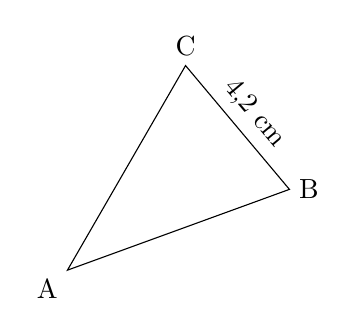
\begin{tikzpicture}[scale=1.5]
    \coordinate[label=below left:A](A)at(0,0);
    \coordinate[label=right:B](B)at(20:2);
    \coordinate[label=C](C)at(60:2);
    \draw(A)--(B)--(C)--cycle;
    \tkzMarkSegment[mark=s||](A,B)
    \tkzMarkSegment[mark=s||](A,C)
    \path(C)--(B)node[above,pos=0.5,sloped]{4,2 cm};
\end{tikzpicture}\hskip15pt
\begin{tikzpicture}[scale=1.5]
    \coordinate[label=above:D](A)at(0,0);
    \coordinate[label=below left:F](B)at(-120:2);
    \coordinate[label=right:G](C)at(-30:2);
    \draw(A)--(B)--(C)--cycle;
    \tkzMarkSegment[mark=s||](A,B)
    \tkzMarkSegment[mark=s||](A,C)
    \tkzMarkRightAngle(B,A,C)
    \path(B)--(A)node[above,pos=0.5,sloped,yshift=10pt]{67 dm};
\end{tikzpicture}\hskip15pt
\begin{tikzpicture}[scale=1.5]
    \coordinate[label=above:H](A)at(0,0);
    \coordinate[label=below left:J](B)at(-140:2);
    \coordinate[label=right:K](C)at(-80:2);
    \draw(A)--(B)--(C)--cycle;
    \tkzMarkSegment[mark=s||](A,B)
    \tkzMarkSegment[mark=s||](A,C)
    \tkzMarkSegment[mark=s||](B,C)
\end{tikzpicture}\hskip15pt
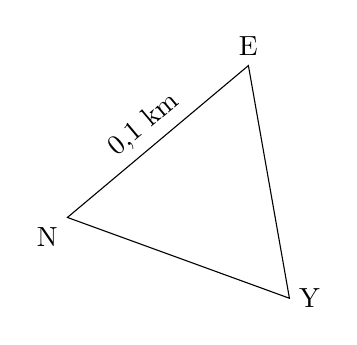
\begin{tikzpicture}[scale=1.5]
    \coordinate[label=above:E](A)at(0,0);
    \coordinate[label=below left:N](B)at(-140:2);
    \coordinate[label=right:Y](C)at(-80:2);
    \draw(A)--(B)--(C)--cycle;
    \path(B)--(A)node[above,pos=0.5,sloped]{0,1 km};
\end{tikzpicture}
\end{document}
